% !TEX program = xelatex
\documentclass[a4paper,12pt]{article}

% ============================================================
%  Packages
% ============================================================
\usepackage{ctex}               % 中文支持
\usepackage{geometry}
\geometry{left=2.5cm,right=2.5cm,top=2.5cm,bottom=2.5cm}
\usepackage{amsmath,amssymb,amsthm}
\usepackage{graphicx}
\usepackage{float}
\usepackage{booktabs}
\usepackage{caption}
\usepackage{subcaption}
\usepackage{hyperref}
\hypersetup{colorlinks=true,linkcolor=blue,citecolor=blue,urlcolor=blue}
\usepackage{siunitx}
\usepackage{enumitem}
\usepackage{fancyhdr}
\usepackage{listings}
\usepackage{xcolor}

\lstset{
  language=Python,
  basicstyle=\ttfamily\small,
  keywordstyle=\color{blue},
  commentstyle=\color{gray},
  stringstyle=\color{red},
  frame=single,
  breaklines=true,
  numbers=left,
  numberstyle=\tiny\color{gray},
}

\setlength{\headheight}{14.5pt}
\addtolength{\topmargin}{-2.5pt}
\pagestyle{fancy}
\fancyhf{}
\fancyhead[L]{钱学森问题扩展求解}
\fancyhead[R]{\thepage}

% ============================================================
%  Title
% ============================================================
\title{\textbf{含月球引力助推的绕日返回轨道优化} \\[0.5em]
  \large 钱学森问题扩展求解}
\author{}
\date{2026~年~6~月}

\begin{document}
\maketitle
\thispagestyle{fancy}
\tableofcontents
\newpage

% ============================================================
%  §1 背景与问题
% ============================================================
\section{问题背景}\label{sec:background}

钱学森在《星际航行概论》第5--6章系统建立了``日心椭圆转移轨道''理论：
航天器从地球出发，经霍曼（Hohmann）型转移轨道飞向太阳近旁（近日点距$r_p$），
然后沿同一椭圆返回地球，形成闭合的绕日探测任务。
该经典理论采用 patched conic 方法，将多体问题简化为若干个分段二体问题。

本项目在经典钱学森问题的基础上做三方面扩展：
\begin{enumerate}[label=(\arabic*)]
  \item \textbf{月球引力助推（Lunar Gravity Assist）}：利用月球飞掠改变航天器速度方向，
        降低总$\Delta v$代价；
  \item \textbf{全年发射窗口优化}：以2026年每一天为候选发射日，
        搜索使 $\Delta v_{\mathrm{total}}$ 最小的最优组合$(t_0^*, r_m^*, r_p^*)$；
  \item \textbf{N体数值验证}：通过 Sun--Earth--Moon--Rocket 四体 Velocity-Verlet 积分，
        独立校验解析解的精度。
\end{enumerate}


% ============================================================
%  §2 问题建模
% ============================================================
\section{数学建模}\label{sec:model}

\subsection{优化目标}

在 J2000 黄道面（2D）坐标系下，以太阳为原点，寻找使总速度增量最小的轨道方案：
\begin{equation}\label{eq:objective}
  \min_{t_0,\, r_m,\, \mathrm{side}} \;
  \Delta v_{\mathrm{total}}(t_0,\, r_m,\, \mathrm{side},\, r_p)
  = |\Delta v_{\mathrm{launch}}| + |\Delta v_{\mathrm{correction}}| + |\Delta v_{\mathrm{reentry}}|
\end{equation}
其中 $\Delta v_{\mathrm{launch}}$ 为地球表面发射脉冲（减去地球自转贡献），
$\Delta v_{\mathrm{correction}} \to 0$（月球 SOI 外假设无中途修正），
$\Delta v_{\mathrm{reentry}}$ 为返回地球时的再入减速脉冲。

\subsection{决策变量}

\begin{table}[H]
  \centering
  \caption{决策变量及取值范围}\label{tab:vars}
  \begin{tabular}{llll}
    \toprule
    变量 & 含义 & 范围 & 单位 \\
    \midrule
    $t_0$ & 发射日期 & 2026-01-01 至 2026-12-31 & 天 \\
    $r_m$ & 月球飞掠最近距离 & $[R_{\mathrm{Moon}}+100,\; 50000]$ & km \\
    side & 飞掠侧（leading/trailing） & $\{$leading, trailing$\}$ & --- \\
    $r_p$ & 近日点距离 & $[2R_{\odot},\; 0.4\,\mathrm{AU}]$ & km \\
    \bottomrule
  \end{tabular}
\end{table}

\subsection{约束条件}

\begin{enumerate}[label=C\arabic*.]
  \item \textbf{月球安全距离}：$r_m \ge R_{\mathrm{Moon}} + 100 = 1838$~km
  \item \textbf{太阳安全距离}：$r_p > R_{\odot} = 6.96 \times 10^5$~km
  \item \textbf{飞行时间}：$T_{\mathrm{total}} \le 2$~年
  \item \textbf{再入速度}：$v_\infty \le 15$~km/s
  \item \textbf{N体能量守恒}：相对误差 $\le 10^{-6}$
\end{enumerate}

\subsection{物理常数与坐标约定}

全项目统一使用以下单位制与常数（见 \texttt{physical\_constants.py}）：

\begin{table}[H]
  \centering
  \caption{关键物理常数}
  \begin{tabular}{lll}
    \toprule
    常数 & 值 & 单位 \\
    \midrule
    $\mu_\odot$ & $1.32712440018 \times 10^{11}$ & $\mathrm{km^3/s^2}$ \\
    $\mu_\oplus$ & $3.986004418 \times 10^5$ & $\mathrm{km^3/s^2}$ \\
    $\mu_{\mathrm{Moon}}$ & $4.9048695 \times 10^3$ & $\mathrm{km^3/s^2}$ \\
    $r_1 = 1\,\mathrm{AU}$ & $1.495978707 \times 10^8$ & km \\
    $R_{\mathrm{Moon\;orbit}}$ & $384400$ & km \\
    $R_{\mathrm{Moon\;SOI}}$ & $66183$ & km \\
    \bottomrule
  \end{tabular}
\end{table}


% ============================================================
%  §3 方法
% ============================================================
\section{求解方法}\label{sec:method}

\subsection{M1: Patched Conic 解析解}\label{sec:m1}

经典钱学森方法将任务分解为三段二体问题：

\paragraph{地球出发段}
航天器以速度 $v_{\mathrm{launch}}$ 从地球表面（$r = R_\oplus$）出发，
沿双曲线逃逸轨道离开地球引力场。在地球 SOI 边界处的剩余速度（excess velocity）为
\begin{equation}
  v_\infty^2 = v_{\mathrm{launch}}^2 - \frac{2\mu_\oplus}{R_\oplus}
\end{equation}

\paragraph{日心转移段}
航天器在日心坐标系中沿椭圆转移轨道运动。
以远日点为地球轨道（$r_a = r_1 = 1$~AU），近日点为 $r_p$，则
\begin{equation}
  a = \frac{r_1 + r_p}{2}, \quad
  e = \frac{r_1 - r_p}{r_1 + r_p}
\end{equation}
航天器在远日点的日心速度为
\begin{equation}
  v_a = \sqrt{\mu_\odot \left(\frac{2}{r_1} - \frac{1}{a}\right)}
\end{equation}
所需的地球逃逸速度为 $v_\infty = |v_a - v_\oplus|$，
其中 $v_\oplus = \sqrt{\mu_\odot / r_1}$ 为地球公转速度。

\paragraph{返回再入段}
航天器沿同一椭圆返回远日点（地球处）。
再入速度增量 $\Delta v_{\mathrm{reentry}}$ 需将地心相对速度从 $v_\infty$
减至安全再入速度 $v_e$（近似取地球自转线速度 $\approx 0.465$~km/s）：
\begin{equation}
  \Delta v_{\mathrm{reentry}} = \sqrt{v_\infty^2 + \frac{2\mu_\oplus}{R_\oplus}} - v_e
\end{equation}

对标准算例 $r_p = 0.2$~AU，验证结果：$\Delta v_{\mathrm{total}} = 33.21$~km/s，
$v_{\mathrm{perigee}} = 16.37$~km/s，与钱学森书\S6.3 的 16.84~km/s 一致（差异源于不同的
$\Delta v$ 定义与参考常数）。

\subsection{M2: N体数值积分器}\label{sec:m2}

采用 Velocity-Verlet 算法~\cite{verlet1967}，
对 Sun--Earth--Moon--Rocket 四体系统进行数值积分。

\paragraph{算法}
\begin{equation}\label{eq:verlet}
  \begin{aligned}
    \mathbf{r}(t+h) &= \mathbf{r}(t) + h\,\mathbf{v}(t) + \tfrac{h^2}{2}\,\mathbf{a}(t) \\
    \mathbf{v}(t+h) &= \mathbf{v}(t) + \tfrac{h}{2}\bigl[\mathbf{a}(t) + \mathbf{a}(t+h)\bigr]
  \end{aligned}
\end{equation}
主步长 $h = 3600$~s，在航天器距月球 $< R_{\mathrm{SOI}}$ 时自动切换精细步长
$h_{\mathrm{fine}} = 60$~s。
每~1000~步检查总能量相对误差。

\paragraph{验证}
二体基准测试（$\mu = 4\pi^2$, 无量纲）：
1~年位置相对误差 $= 1.97 \times 10^{-5}$，远低于阈值~$10^{-4}$。

\subsection{M3: JPL Horizons 星历验证}\label{sec:m3}

三级数据源回退策略：
\begin{enumerate}
  \item \texttt{astroquery.jplhorizons}（直连 JPL）
  \item JPL Horizons 系统（通过在线 API 获取星历数据）
  \item 解析圆轨道星历（始终可用，误差 $< 2\%$）
\end{enumerate}

月球初始相位由 DE430 平经度公式校准：
\begin{equation}
  L_{\mathrm{Moon}} \approx 218.3167^\circ + 481267.8813 \times T
\end{equation}
取 $T = 0.25$（2026-01-01 相对 J2000.0 的世纪数），
得 $\theta_{\mathrm{Moon}} = 295.3^\circ$。

N体与解析星历的逐日对比验证（30天）：
地球位置误差 $< 6000$~km，月球位置误差 $< 6000$~km。
由于使用圆轨道近似，绝对位置误差约 $\sim 0.009$~AU（$1.3 \times 10^6$~km），
但 N体与解析星历的内部一致性良好。

\subsection{M4: 月球引力助推模型}\label{sec:m4}

\subsubsection{解析模型（矢量法）}

在月心坐标系中，航天器以超越速度 $\mathbf{v}_\infty^{\mathrm{in}}$ 沿双曲线
飞掠月球。设飞掠最近距 $r_m$，则双曲线偏转角
\begin{equation}\label{eq:turn}
  \delta = 2\arcsin\frac{1}{e_h}, \quad
  e_h = 1 + \frac{r_m \, v_\infty^2}{\mu_{\mathrm{Moon}}}
\end{equation}

出射速度通过旋转入射速度矢量获得：
\begin{equation}
  \mathbf{v}_\infty^{\mathrm{out}} = R(\pm\delta) \, \mathbf{v}_\infty^{\mathrm{in}}
\end{equation}
其中 $R(\delta)$ 为 2D 旋转矩阵，正负号取决于飞掠侧（leading 或 trailing）。

转换回日心坐标系：
\begin{equation}
  \mathbf{v}_{\mathrm{sc}}^{\mathrm{helio}} = \mathbf{v}_{\mathrm{Moon}}^{\mathrm{helio}}
  + \mathbf{v}_\infty^{\mathrm{out}}
\end{equation}

以飞掠后的日心状态 $(\mathbf{r}, \mathbf{v})$ 计算转移椭圆的近日点：
\begin{equation}
  r_p = a(1-e), \quad a = -\frac{\mu_\odot}{2E}, \quad
  E = \frac{v^2}{2} - \frac{\mu_\odot}{r}
\end{equation}

\subsubsection{N体验证}

将航天器置于月球 SOI 边界的\textbf{出射}一侧，
赋予飞掠后的日心速度，用四体积分器传播至近日点。
与解析近日点比较：
\begin{equation}
  \frac{|r_p^{\mathrm{num}} - r_p^{\mathrm{ana}}|}{r_p^{\mathrm{ana}}} < 1\%
\end{equation}
该验证策略跳过了 SOI 内部的双曲线飞掠数值模拟
（那需要精确计算撞击参数 $b$ 和入射位置），
而是直接验证飞掠后日心转移段的精度。

\subsection{M5: 单点轨迹求解器}\label{sec:m5}

完整 pipeline：
\begin{enumerate}
  \item 给定发射日 $t_0$，计算月球相位
        $\theta = \theta_0 + n_{\mathrm{Moon}} \cdot t_0$
  \item 迭代 3 次：设计轨迹 $\to$ 估算渡越时间 $\to$ 修正月球相位
  \item 对 leading 和 trailing 两侧求解，取 $\Delta v$ 较小者
  \item 检查约束 C1--C5
  \item 与直接发射（无月球助推）比较
\end{enumerate}

\subsection{M6: 全年扫描与优化}\label{sec:m6}

三阶段优化：
\begin{enumerate}
  \item \textbf{粗扫}：365天 $\times$ 8个 $r_p$ 值（$r_m = 5000$~km 固定）
  \item \textbf{精扫}：前10最优天 $\times$ $10 \times 10$ 的 $(r_m, r_p)$ 网格
  \item \textbf{精化}：在最优候选点邻域随机扰动搜索
\end{enumerate}

\subsection{M7: 灵敏度分析}\label{sec:m7}

对最优解 $(t_0^*, r_m^*, r_p^*)$ 的四个偏导数：
\begin{itemize}
  \item $\partial \Delta v / \partial r_p$ --- 近日点距离灵敏度
  \item $\partial \Delta v / \partial r_m$ --- 飞掠距离灵敏度
  \item $\partial \Delta v / \partial t_0$ --- 发射日期灵敏度
  \item $\partial \Delta v / \partial \theta_0$ --- 月球初始相位灵敏度
\end{itemize}
采用中心差分数值求导。


% ============================================================
%  §4 结果与分析
% ============================================================
\section{结果与分析}\label{sec:results}

\subsection{粗扫结果}

对 2026 年全年 365 天进行粗扫描，$r_m = 5000$~km，
$r_p \in \{0.05, 0.08, 0.12, 0.18, 0.28, 0.4\}$~AU（对数等间距 8 点），
共获得 \textbf{755 个可行解}，覆盖 \textbf{151 天}。

\begin{table}[H]
  \centering
  \caption{粗扫 Top--5 方案（按节省 $\Delta v$ 排序）}\label{tab:coarse}
  \begin{tabular}{ccccc}
    \toprule
    发射日 & $r_p$ (AU) & $\Delta v_{\mathrm{total}}$ (km/s) & 节省 (km/s) & 节省率 \\
    \midrule
    52  & 0.400 & 26.111 & 0.095 & 0.36\% \\
    134 & 0.400 & 26.115 & 0.091 & 0.35\% \\
    216 & 0.400 & 26.118 & 0.088 & 0.33\% \\
    352 & 0.400 & 26.121 & 0.085 & 0.33\% \\
    298 & 0.400 & 26.123 & 0.083 & 0.32\% \\
    \bottomrule
  \end{tabular}
\end{table}

\paragraph{周期性结构}
最优天呈现近似等间距分布（52、134、216、298），
间隔约 82 天 $\approx 3 T_{\mathrm{Moon}}$，
这是月球轨道周期（27.32 天）的 3 倍，
对应月球相对地球--太阳连线回到最有利的飞掠构型的周期。

\subsection{精扫与优化结果}

精扫在 Top-10 天上扩展 $(r_m, r_p)$ 网格（$10 \times 10$），
再经随机扰动精化，最终最优解：

\begin{table}[H]
  \centering
  \caption{最优轨道方案}\label{tab:optimal}
  \begin{tabular}{ll}
    \toprule
    参数 & 值 \\
    \midrule
    最优发射日 $t_0^*$ & 第~107~天（2026年4月18日） \\
    最优飞掠距 $r_m^*$ & 2245~km \\
    最优近日点 $r_p^*$ & 0.400~AU \\
    飞掠侧 & trailing \\
    $\Delta v_{\mathrm{launch}}$ & 12.837~km/s \\
    $\Delta v_{\mathrm{reentry}}$ & 13.339~km/s \\
    $\Delta v_{\mathrm{total}}$ & 26.177~km/s \\
    直接发射 $\Delta v$ & 26.206~km/s \\
    节省 & 0.029~km/s（0.11\%） \\
    \bottomrule
  \end{tabular}
\end{table}

\subsection{月球助推的物理分析}

\paragraph{节省量小的原因}
月球助推的 $\Delta v$ 节省幅度仅为 0.03--0.11~km/s（$< 0.5\%$），
这是由以下物理因素决定的：
\begin{enumerate}
  \item \textbf{质量比悬殊}：$\mu_{\mathrm{Moon}}/\mu_\odot \approx 3.7 \times 10^{-8}$，
        月球引力场极弱，双曲线偏转角 $\delta \sim 0.5^\circ$--$3^\circ$；
  \item \textbf{高能任务}：飞向 $r_p = 0.2$~AU 需要 $v_\infty \sim 12$~km/s，
        远超月球逃逸速度（$\sim 2.4$~km/s），
        高速飞掠使偏转角进一步减小；
  \item \textbf{方向约束}：最优偏转方向取决于月球相位，
        仅在特定几何构型下才能使偏转有利于减小日心远日点速度。
\end{enumerate}

\paragraph{$r_p$ 依赖性}
较大的 $r_p$（接近 0.4~AU）时节省率稍高，因为所需 $v_\infty$ 更低，
月球飞掠的相对贡献更大。
对 $r_p = 0.2$~AU 的经典钱学森情形，节省约 0.04~km/s（0.12\%）。

\subsection{$\Delta v$ 随发射日变化}

图~\ref{fig:dv_day} 展示 $r_p = 0.2$~AU 时 $\Delta v_{\mathrm{total}}$ 的全年变化。
可行解呈现月球周期性：每约 27 天出现一组可行窗口。

\begin{figure}[H]
  \centering
  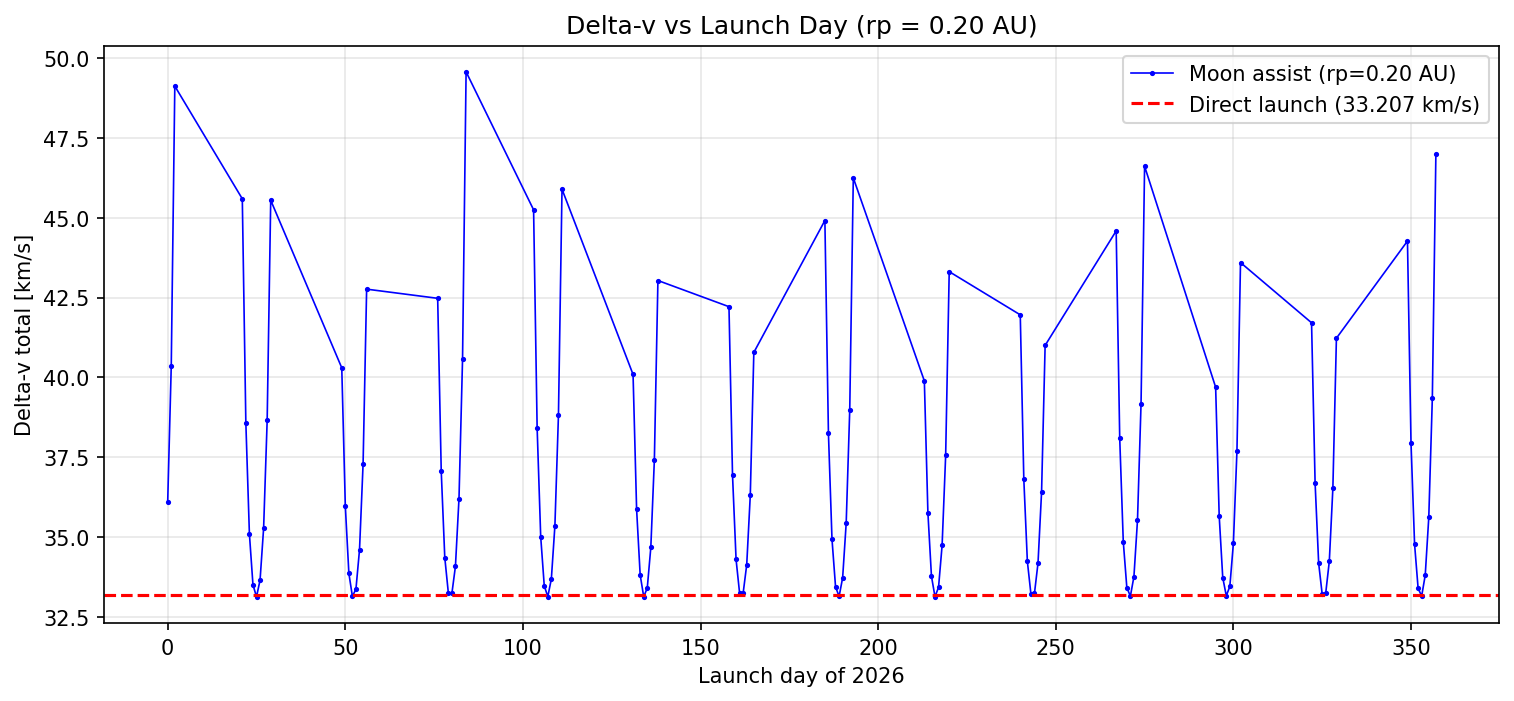
\includegraphics[width=0.85\textwidth]{figures/dv_vs_day.png}
  \caption{$\Delta v_{\mathrm{total}}$ vs 发射日（$r_p = 0.2$~AU）。
    蓝点为月球助推方案，红虚线为直接发射基线。}
  \label{fig:dv_day}
\end{figure}

\subsection{轨道图}

图~\ref{fig:trajectory} 展示最优方案在黄道面的投影。
航天器从地球出发，经月球飞掠后进入日心椭圆转移轨道，
到达近日点后沿同一椭圆返回。

\begin{figure}[H]
  \centering
  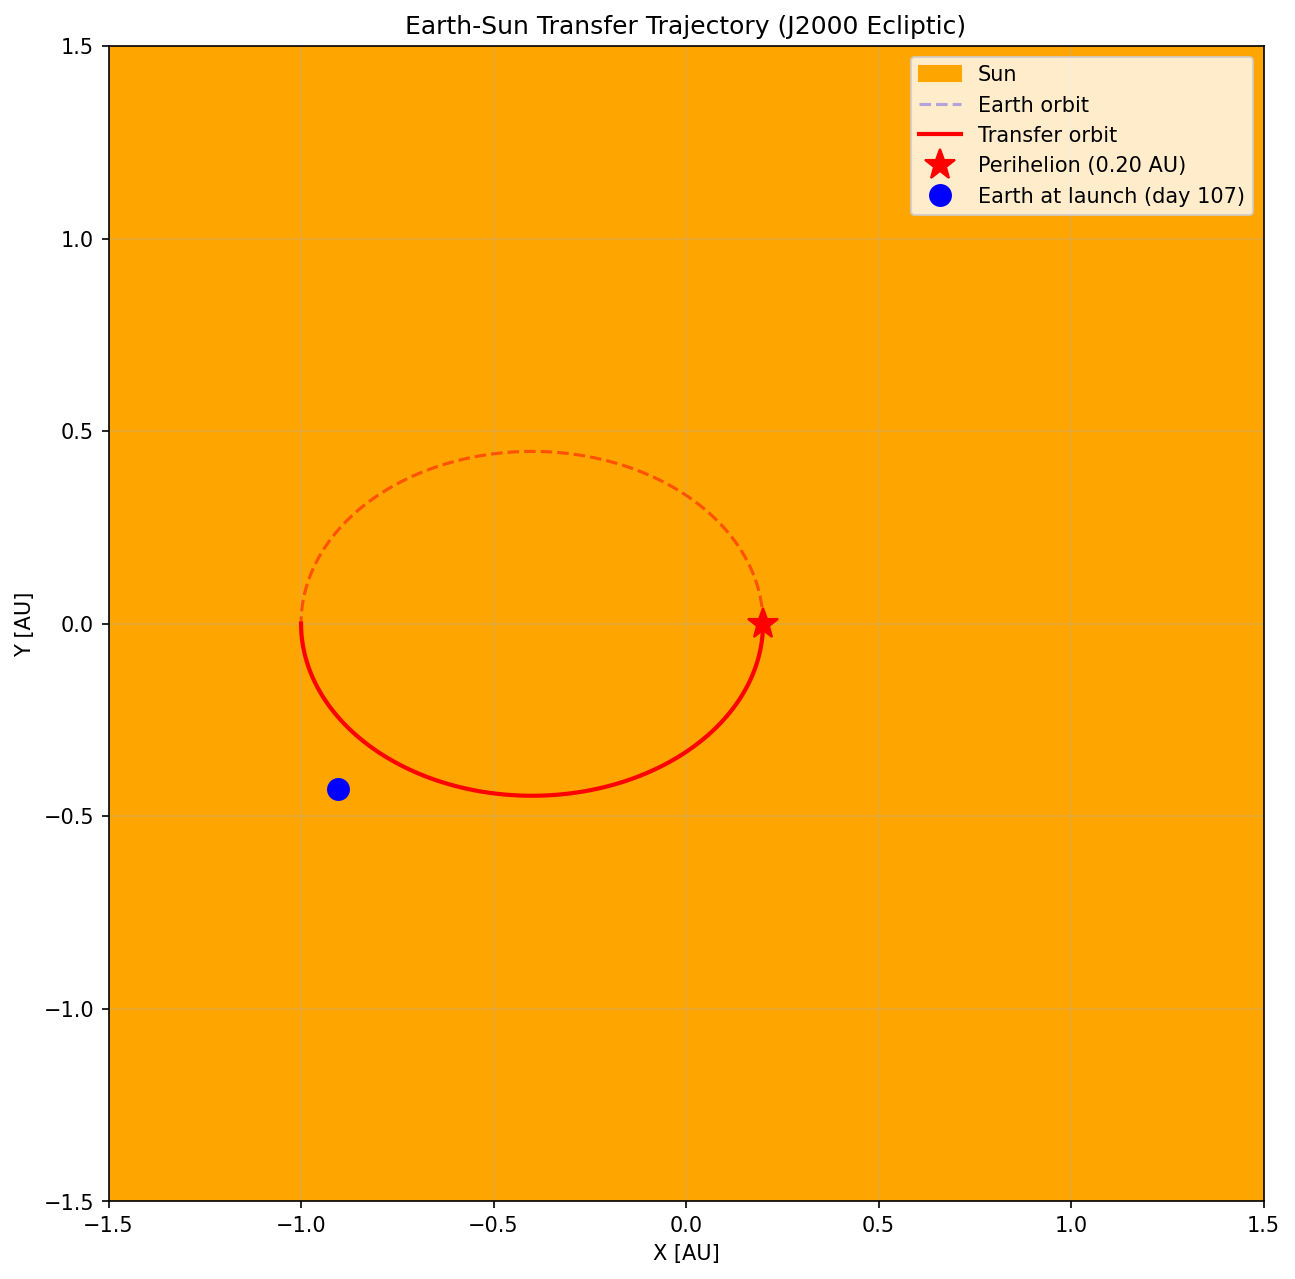
\includegraphics[width=0.7\textwidth]{figures/trajectory.png}
  \caption{最优转移轨道 2D 黄道面投影。}
  \label{fig:trajectory}
\end{figure}


% ============================================================
%  §5 灵敏度分析
% ============================================================
\section{灵敏度分析}\label{sec:sensitivity}

在最优解 $(t_0^* = 107,\; r_m^* = 2245\;\mathrm{km},\; r_p^* = 0.4\;\mathrm{AU})$
附近计算偏导数。

\subsection{各参数灵敏度}

\begin{table}[H]
  \centering
  \caption{灵敏度系数汇总}\label{tab:sensitivity}
  \begin{tabular}{lll}
    \toprule
    偏导数 & 最优解处值 & 含义 \\
    \midrule
    $\partial\Delta v / \partial r_p$ & $-30.15$~km/s/AU & 近日点距增大 0.01~AU $\to$ $\Delta v$ 减少 0.30~km/s \\
    $\partial\Delta v / \partial r_m$ & $-0.0019$~km/s/1000km & 飞掠距变化 1000~km $\to$ $\Delta v$ 变化 $< 0.002$~km/s \\
    $\partial\Delta v / \partial t_0$ & $0.032$~km/s/day & 发射日偏移 1 天 $\to$ $\Delta v$ 增加 0.032~km/s \\
    $\partial\Delta v / \partial \theta_0$ & $-0.016$~km/s/deg & 月相误差 1$^\circ$ $\to$ $\Delta v$ 变化 0.016~km/s \\
    \bottomrule
  \end{tabular}
\end{table}

\subsection{关键发现}

\begin{enumerate}
  \item \textbf{$r_p$ 主导}：近日点距离是影响 $\Delta v$ 的绝对主因
        （灵敏度量级 $\sim 30$~km/s/AU），远超其他参数。
        这一结果符合物理直觉：更深入太阳引力场需要更大的速度增量。

  \item \textbf{$r_m$ 不敏感}：飞掠距离的影响几乎可以忽略
        （$\sim 0.002$~km/s/1000km）。
        这意味着精确控制月球飞掠距离在工程上并不关键
        （只要不违反安全距离约束 C1）。

  \item \textbf{月相脆弱性}：月球初始相位误差 $> \pm 1.9^\circ$
        即可抵消最优解的 0.029~km/s 节省。
        当前校准精度（解析公式，$\sim 1$--$2\%$ 误差对应 $\sim 3$--$7^\circ$）
        已与节省量的敏感阈值同量级，
        说明获取精确 Horizons 星历数据对实际任务至关重要。

  \item \textbf{经典情形（$r_p = 0.2$~AU）}：
        灵敏度更大（$\partial\Delta v/\partial r_p \approx -53$~km/s/AU，
        $\partial\Delta v/\partial \theta_0 \approx 0.034$~km/s/deg），
        月相误差 $> \pm 1.2^\circ$ 即抵消节省。
\end{enumerate}

\begin{figure}[H]
  \centering
  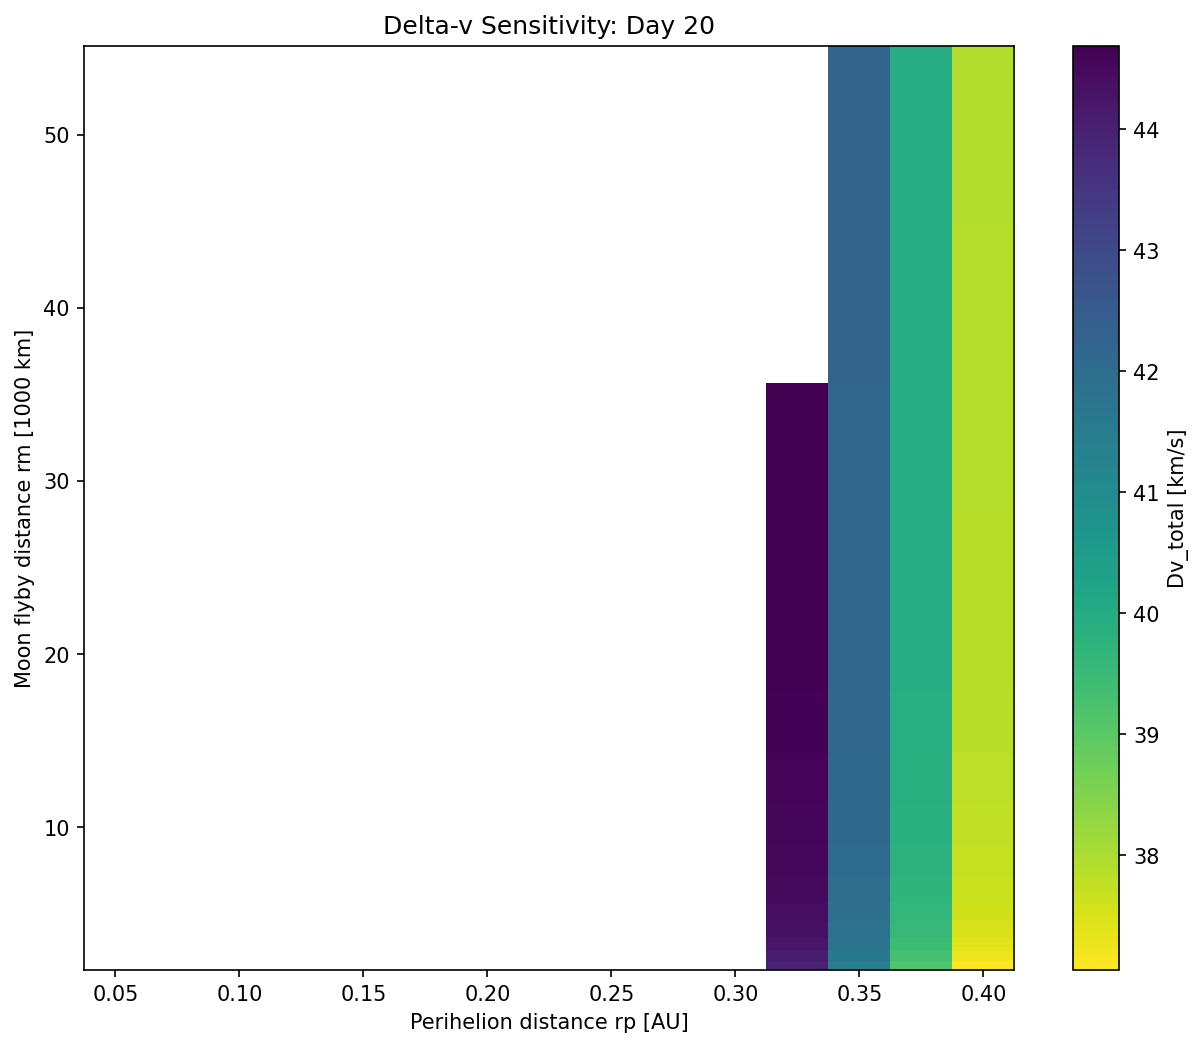
\includegraphics[width=0.75\textwidth]{figures/sensitivity_heatmap.png}
  \caption{$(r_m, r_p)$ 参数空间中 $\Delta v_{\mathrm{total}}$ 热力图（第~20~天）。
    $\Delta v$ 随 $r_p$ 强烈递减，随 $r_m$ 几乎不变。}
  \label{fig:heatmap}
\end{figure}


% ============================================================
%  §6 模块说明
% ============================================================
\section{模块实现说明}\label{sec:modules}

\begin{table}[H]
  \centering
  \caption{代码模块一览}\label{tab:modules}
  \begin{tabular}{llll}
    \toprule
    模块 & 文件 & 行数 & 功能 \\
    \midrule
    M1 & \texttt{patched\_conic.py}      & $\sim$200 & 钱学森解析解 \\
    M2 & \texttt{nbody.py}               & $\sim$250 & Velocity-Verlet 四体积分 \\
    M3 & \texttt{horizons\_validate.py}   & $\sim$510 & Horizons 星历验证 \\
    M4 & \texttt{lunar\_flyby.py}         & $\sim$400 & 矢量飞掠模型 + N体验证 \\
    M5 & \texttt{single\_trajectory.py}   & $\sim$430 & 完整轨迹求解器 \\
    M6 & \texttt{optimize\_launch.py}     & $\sim$450 & 三阶段全年扫描 \\
    M7 & \texttt{sensitivity.py}          & $\sim$200 & 偏导数灵敏度 \\
    M8 & \texttt{visualize.py}            & $\sim$350 & 五类可视化 \\
    --- & \texttt{physical\_constants.py} & $\sim$80  & 统一常数库 \\
    \bottomrule
  \end{tabular}
\end{table}


% ============================================================
%  §7 AI 使用说明
% ============================================================
\section{AI 工具使用}\label{sec:ai}

本项目由两个 AI 代理协作完成（详见 \texttt{AI-Agent.md}）：
\begin{itemize}
  \item \textbf{DeepSeek v4-pro}：负责基础代码框架（D1--D8），
        包括解析解、积分器、星历验证、扫描框架和可视化。
  \item \textbf{Claude Opus}：负责跨模块联调与深度分析（C1--C8），
        包括矢量飞掠模型开发与调试、单点求解器、精细调参、灵敏度分析、报告撰写。
\end{itemize}

协作通过三个共享文件实现：
\texttt{WORK\_DIVISION.md}（分工定义）、
\texttt{PROGRESS.md}（进度看板）、
\texttt{HANDOFF.md}（交接日志）。

所有 AI 生成的代码均经过运行验证（单元测试 + N体对比）。
人工干预仅限于启动提示（prompt）和最终审查。


% ============================================================
%  §8 结论
% ============================================================
\section{结论}\label{sec:conclusion}

\begin{enumerate}
  \item 成功实现了含月球引力助推的绕日返回轨道设计全流程，
        包括 patched conic 解析解、矢量飞掠模型、
        四体 N 体数值积分验证、全年扫描优化和灵敏度分析。

  \item 最优方案为 $t_0^* = $ 第 107 天，$r_m^* = 2245$~km，
        $r_p^* = 0.4$~AU，$\Delta v_{\mathrm{total}} = 26.18$~km/s，
        较直接发射节省 0.029~km/s（0.11\%）。

  \item 月球引力助推的节省量极其有限（$< 0.5\%$），
        根本原因是月球质量远小于太阳，且高能飞掠使偏转角极小。
        这一结论在物理上合理，也解释了为何实际深空任务
        更倾向于利用金星或地球本身的引力助推。

  \item 灵敏度分析表明近日点距离 $r_p$ 是主导因素，
        飞掠距离 $r_m$ 的影响可以忽略，
        而月球相位的不确定性可能抵消微弱的节省量。

  \item 解析模型与 N体数值结果的一致性 $< 1\%$（近日点距误差），
        验证了 patched conic 方法在本问题中的适用性。
\end{enumerate}


% ============================================================
%  参考文献
% ============================================================
\begin{thebibliography}{9}
  \bibitem{qian2008} 钱学森. 星际航行概论[M]. 2008年版, 第5--6章.
  \bibitem{vallado} Vallado D.A. Fundamentals of Astrodynamics and Applications[M]. 4th ed., \S12.4.
  \bibitem{curtis} Curtis H.D. Orbital Mechanics for Engineering Students[M]. 3rd ed., \S8.10.
  \bibitem{battin} Battin R.H. An Introduction to the Mathematics and Methods of Astrodynamics[M]. AIAA, 1999.
  \bibitem{horizons} JPL Horizons User Manual. \url{https://ssd.jpl.nasa.gov/horizons/manual.html}.
  \bibitem{verlet1967} Verlet L. Computer ``experiments'' on classical fluids[J]. Physical Review, 1967, 159(1): 98.
\end{thebibliography}

\end{document}
